\section{Journey to the Center of the Mind}

\begin{quotex}
The spiritual adepts were inner-world adventurers of the highest daring, the Tibetan equivalent of our astronauts—I think it is worth coining the term `psychonaut' to describe them. They personally voyaged to the furthest frontiers of that universe which their society deemed vital to explore: the inner frontiers of consciousness itself, in all its transformations in life and beyond death. \flright{\textsc{Huston Smith}, Introduction to \emph{The Tibetan Book of the Dead}}

It should be clear that the theory behind the use of enthogens for spiritual ``enlightenment" is deeply flawed. It assumes that such enlightenment involves a particular experience, or set of experiences, that are somehow to be distinguished from all other experiences. This idea comes from the confusion of the psychic and the spiritual. \flright{\textsc{Rene Guenon}, \emph{The Reign of Quantity}}

The idea that hallucinogens could produce a transcendental experience is shocking. The drug merely uncovers the normally unconscious functional layer of perceptional and emotional variants, which are psychologically transcendent, but by no means ``transcendental", i.e. — metaphysical. \flright{\textsc{Carl Jung}}

Knowledge is a function of being. When there is a change in the being of the knower, there is a corresponding change in the nature and amount of knowing. \flright{\textsc{Aldous Huxley}, \emph{The Perennial Philosophy}}

\end{quotex}

\paragraph{The Doors of Perception}

Aldous Huxley was a popularizer of the so-called Perennial Philosophy, a term first coined by Leibniz. In his book of that same title, he introduced several topics supported with extensive quotes from mystics and sages of several Traditions. This has two benefits to the reader:

\begin{itemize}
\item To pick out the highlights of the various traditions. At its best, the quotes should encourage readers to learn more about the topic. At its worst, it provides quotes to be repeated on social media to create the spectacle of wisdom. 
\item By pointing out similar notions from different traditions, it shows that these topics have some objective validity and are not matters of blind faith to specific religions. 
\end{itemize}
Unfortunately for Huxley, the mere repetition of beautiful and enticing quotes does not a mystic make. He seems not to have followed a specific tradition. Moreover, there is a shadow side to the Perennial Philosophy. Bad things can happen and humans are subject to malevolent influences. As he points out, knowledge requires a change in being, and that change requires purifications of the mind, will, and emotions.

That sounds difficult, so Huxley looked for a shortcut. In \emph{Doors of Perception}, he describes his experiences with psychedelic substances. It is impossible for chemicals to create a change in being that he is seeking. That is because consciousness and intellect transcend the material world and thus cannot be changed by any material cause. Quite the contrary, intellectual knowledge brackets out the world of the senses in a series of abstractions.

\begin{wrapfigure}{rt}{.3\textwidth}
 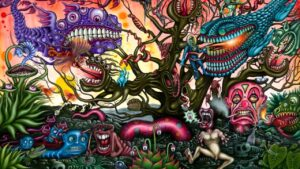
\includegraphics[scale=.5]{a20210923JourneytotheCenteroftheMind-img001.jpg} 
\end{wrapfigure}

Nevertheless, he persisted on his own course. Even when he was suffering severely from cancer, on his deathbed he was administered large doses of LSD by his wife. She describes his death as very peaceful, something confirmed by the medical professionals standing by. However, it is not obvious that death should be easy nor that fear is unnatural. Certainly, on the other side, life is not necessarily butterflies and lollipops. Au contraire, had Huxley paid closer attention to his sources, he should have noticed that.

A very wise friend recently explained to me that fear and pain should not always be hidden with drugs. For example, professional musicians often use beta blockers to slow down their heart rates before a performance. For example, performing on stage is like confronting the fear of death; the solution is to recognize it as the illusion it is. Midwives discourage the use of epidural anesthesia, claiming that the avoidance of pain turns the mother into a zombie.

\paragraph{Exploring Inner Space}
Timothy Leary was a psychology professor at Harvard, doing experiments with LSD. Apparently, things got out of hand. He and his colleague Richard Alpert, NKA Ram Dass, were dismissed from their positions.

Leary continued on as a prophet of some sort, encouraging seeks to explore the new frontier of Inner Space, rather than the more glamorous Outer Space. He used the \emph{Tibetan Book of the Dead} as a guide to help those on LSD trips. His life took some rather colorful turns, as he got in trouble with the law once LSD was criminalized. You can look that up on your own. He was also a model for a resuscitated Order of the Golden Dawn.

Ram Dass, a graduate of my alma mater, went off on a more mystical direction. He embraced Oriental spiritual teachings and also those of Alice Bailey who claimed to have channeled advanced teachings from a Tibetan master. Since I was enamored by anything Tibetan at that time, I ate it all up.

\paragraph{Better Living through Chemistry}
Decades after Huxley and Leary, it has all come to naught. They left behind nothing but a set of aspirations. At that time, their chemically aided spiritual quest was intended for intellectuals competent to understand the truly valid traditional teachings that they knew. There was a genuine desire for spiritual enlightenment; entheogens were not used for pleasure nor to deaden pain, but rather, naively in retrospect, to bring enlightenment.

Since the world of experience is a sensual representation of it in consciousness, these psychedelic drugs distort that psychical process. Hence, the conclusion seems to be that our collective representations of the world are rather arbitrary. In a sense, that is perfectly true, although chemicals won't bring us to the correct representation. Better living through chemistry does not apply to metaphysical teachings.

Now that drug usage has become the sport of the masses, it has lost its allure. There is no pretense of seeking any sort of enlightenment. Rather than the boom for humanity that the early adopters assumed, drugs are a bane, causing addiction, misery, and premature death. Obviously, if drugs truly are the shortcut to mystical knowledge, then the USA would be the most enlightened country on Earth. The evidence is just the opposite.

\paragraph{The Spiritual Quest}
So that's how I started the journey to the center of the mind. I can tell you strange stories, but for now I'll keep them private. It turned into a lifelong project with some occasional interruptions due both to temptations and the years spent as a householder. In a short time, I embraced a more sold path, leaving the chemical brothers as an old memory. Only 3 knights who set out on the quest were able to reach the Holy Grail. So there is little reason to be hopeful about all the noisy parties posting useless advice on social media.

There is no Yellow Brick Road for the Knight to follow. Rather he has to start from wherever he is, not where he should be. Nor is the destination marked; it requires a process of trial and error.

A Knight does not choose his battles; rather he has to the fight the battles that come to him.

Art works: \url{https://www.youtube.com/watch?v=1qNrAB-mNww}

\flrightit{Posted on 2021-09-23 by Cologero }

\begin{center}* * *\end{center}

\begin{footnotesize}\begin{sffamily}



\texttt{Ismo Meinander on 2021-09-24 at 05:57 said: }

You too have been enamored by Bailey? I ingested her works in the past also. Channeling seems to be the new theosophy. I have no doubts about mental telepathy, but I very much doubt Bailey's advanced knowledge nowadays and stay out of it.

I have been addicted to cannabis since 16 years old. I left it behind for years only to find myself again ingesting the substance; despair and insomnia were two reasons for coming back to usage. Only lately I have been able to leave it behind, and I feel like born again. What a wretched being I was about to become.


\hfill

\texttt{veritycacciatrice on 2021-09-24 at 17:03 said: }

I enjoyed Huxley's `Door's'. it was colourful, but as synthetic as `Fear and Loathing' and `On the Road.'

About 15 years ago someone gifted me a signed copy of `House of Leaves.' Not my usual taste but what the heck.

`Leaves' is literally a journey to the centre of the protagonists mind, with parallel tales of those who went mad in the same space using the metaphor of a strange black house, its shifting and dark internal space, and its exploration.

It's en par with Huxley, Thompson et al., not that it's a peer of those genres (nor generation), yet as far as `journey to the centre of the mind' goes, it absolutely is.

What I took from it was that one must employ courage and will in driving thoughts to their logical destination at the farthest branch of an idea, because one may descend into black madness if one stops from fear, or leaps chemically from one `twig' to the other without the benefit of pre-prepared, intellectual `weight-bearing' branches. But if carried all the way one ought find a comfortable corner of Reality where sleep is healthy and sound.

Hell is a great way to flesh out the corridors of a mind to see where the `house-owner' ends up. Mad? Addicted? Lonely? Smiling at God with the sun on their face?

I'm sleeping well these days.


\end{sffamily}\end{footnotesize}
